% Figure 4: Multi-Agent Framework Performance Comparison
\begin{figure}[htbp]
\centering
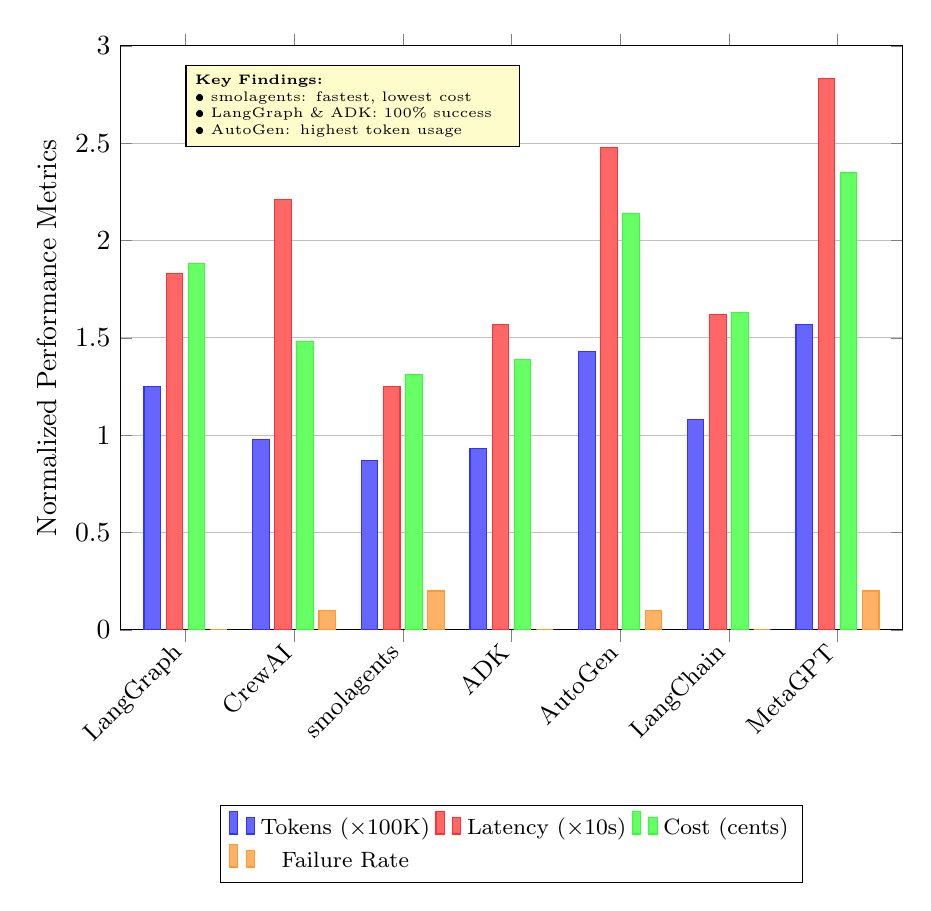
\begin{tikzpicture}
\begin{axis}[
    ybar,
    width=0.95\textwidth,
    height=9cm,
    ylabel={Normalized Performance Metrics},
    symbolic x coords={LangGraph,CrewAI,smolagents,ADK,AutoGen,LangChain,MetaGPT},
    xtick=data,
    xticklabel style={rotate=45, anchor=east, font=\small},
    legend style={at={(0.5,-0.3)}, anchor=north, legend columns=3, font=\footnotesize},
    ymajorgrids=true,
    bar width=6pt,
    ymin=0,
    ymax=3.0,
    enlarge x limits=0.1,
]

% Normalized tokens (÷100 to fit scale)
\addplot[fill=blue!60, draw=blue!80] coordinates {
    (LangGraph,1.25) (CrewAI,0.98) (smolagents,0.87) 
    (ADK,0.93) (AutoGen,1.43) (LangChain,1.08) (MetaGPT,1.57)
};

% Normalized latency (÷10 to fit scale)
\addplot[fill=red!60, draw=red!80] coordinates {
    (LangGraph,1.83) (CrewAI,2.21) (smolagents,1.25) 
    (ADK,1.57) (AutoGen,2.48) (LangChain,1.62) (MetaGPT,2.83)
};

% Cost (in cents)
\addplot[fill=green!60, draw=green!80] coordinates {
    (LangGraph,1.88) (CrewAI,1.48) (smolagents,1.31) 
    (ADK,1.39) (AutoGen,2.14) (LangChain,1.63) (MetaGPT,2.35)
};

% Success rate (÷100 to fit scale, inverted so lower is better)
\addplot[fill=orange!60, draw=orange!80] coordinates {
    (LangGraph,0.0) (CrewAI,0.10) (smolagents,0.20) 
    (ADK,0.0) (AutoGen,0.10) (LangChain,0.0) (MetaGPT,0.20)
};

\legend{Tokens ($\times$100K), Latency ($\times$10s), Cost (cents), Failure Rate}

% Add annotation
\node[draw, fill=yellow!20, text width=4cm, align=left, font=\tiny, anchor=north west] 
    at (axis cs:LangGraph,2.9) {
    \textbf{Key Findings:}\\
    • smolagents: fastest, lowest cost\\
    • LangGraph \& ADK: 100\% success\\
    • AutoGen: highest token usage
};

\end{axis}
\end{tikzpicture}
\caption{Multi-agent framework performance comparison on Au$_{13}$ nanocluster pipeline. Lower values indicate better performance for all metrics. smolagents achieves lowest token usage (87K) and latency (12.5s), while LangGraph and Google ADK offer best reliability (100\% success rate). See Table~\ref{tab:frameworks} for detailed values.}
\label{fig:performance}
\end{figure}
